% Template; to be used with:
%          spconf.sty  - ICASSP/ICIP LaTeX style file, and
%          IEEEbib.bst - IEEE bibliography style file.
% --------------------------------------------------------------------------
\documentclass{article}
\usepackage{spconf,amsmath,graphicx}
\usepackage{booktabs}   % professional table rules
\usepackage{pgfplots}   % bar charts
\usepackage{pgfplotstable}
\pgfplotsset{compat=1.18}
\usepackage{amsmath}    % for \text{} inside equations
\usepackage{multirow}   % optional, for merged table cells
\usepackage{tikz}
\usepackage{url}
\usetikzlibrary{arrows.meta,positioning}
\usetikzlibrary{calc}
\usetikzlibrary{patterns}

% Example definitions.
% --------------------
\def\x{{\mathbf x}}
\def\L{{\cal L}}

% Title.
% ------
\title{TikTalk: A Generative AI-based Oral Language Practice System for Children}
%
% Single address.
% ---------------
\name{JiaJia Liu,  Liwen Ke,  Jiecheng Zheng,  Jiakun Shang,  Guotao Yu (Group09)}
\address{NUS-ISS, National University of Singapore, Singapore 119615}

\begin{document}
%\ninept
%
\maketitle
%

\begin{abstract}

The abstract should consist of one paragraph describing the motivation for your project and a high-level explanation of the methodology you used and the results obtained. Note: this \textit{two-column} project report template is modified from that used in Stanford University CS230, https://cs230.stanford.edu/. 

\end{abstract}
%

\textbf{Keywords}: Please provide (up to four) keywords

\section{Introduction}
\label{sec:intro}

Explain the problem statement and why it is important. Add one paragraph to clearly state the highlights (i.e., the selling point) of your project.

\section{Literature review}
Present relevant references (e.g., papers, industrial products), and discuss their strengths and weaknesses.

\section{Proposed approach}
Describe your proposed system. Use a system architecture or flowchart to illustrate your proposed system. For each module, give a detailed description of how it works.

\subsection{System Overview}
\subsection{Diffusion Module}
\label{sec:diffusion}

The diffusion module sits at the head of the TikTalk pipeline and is
responsible for producing the visual stimulus that drives the entire
oral-practice loop. Because every downstream module — VLM ground-truth
generation, ASR, and scoring — consumes the image (or its derived
description) produced here, the quality, semantic clarity, and stylistic
consistency of the generated image directly upper-bound the quality of
the whole system.

The final system adopts OpenAI's
\textit{DALL-E~3}~\cite{betker2023dalle3} as the text-to-image backbone
and surrounds it with a deterministic three-layer
\textit{prompt-assembly} pipeline that is engineered specifically for
the Primary~School~Leaving~Examination (PSLE)
Stimulus-Based-Conversation~(SBC) task. The choice of an API-based
diffusion backbone over a locally fine-tuned alternative is a
deliberate engineering trade-off discussed in
Section~\ref{sec:diffusion-backbone}.

\subsubsection{Role in the TikTalk Pipeline}
\label{sec:diffusion-role}

Within the end-to-end TikTalk pipeline, the diffusion
module is invoked first: a structured user selection (or a free-form
prompt) is translated into a final text prompt, sent to DALL-E~3, and
the returned PNG is forwarded — together with its accompanying prompt
metadata — to the VLM module for ground-truth caption generation. The
generated image therefore plays two roles simultaneously: it is the
visual stimulus shown to the student in the front-end, and it is the
single source of truth from which the system later derives the
ground-truth description used by the scoring module. Any ambiguity or
visual clutter in the image is propagated, amplified, and ultimately
penalised at the scoring stage. We therefore impose three
non-negotiable design constraints on every generated image:
(i)~\textbf{semantic clarity} — the scene must contain a small number of
clearly identifiable objects and actions; (ii)~\textbf{describability} —
the visual content must be expressible in the vocabulary and grammar of
a 6--12-year-old Singaporean primary-school student; and
(iii)~\textbf{stylistic uniformity} — every image must look like a page
from a children's storybook so that the visual register is consistent
across sessions.

\subsubsection{Backbone Selection: From Foundation Models to Local
Fine-Tuning}
\label{sec:diffusion-backbone}

Text-to-image generation in 2024--2026 splits into two architecturally
distinct routes: (a)~closed-source \textbf{foundation T2I APIs} that
expose a large, frozen model behind a single HTTP boundary --- DALL-E~3
\cite{betker2023dalle3}, Imagen~3~\cite{imagenteam2024imagen3}, Midjourney;
and (b)~open-weight backbones --- SDXL~\cite{podell2023sdxl},
Stable~Diffusion~3~\cite{esser2024sd3}, FLUX.1~\cite{bfl2024flux} ---
that can be hosted locally and \textit{domain-adapted} via
parameter-efficient adapters such as LoRA~\cite{hu2022lora}. We
evaluated both routes seriously before adopting DALL-E~3 with prompt
engineering as the production backbone.

\noindent\textbf{Why a foundation T2I model.}
Modern foundation T2I models offer three properties that match the
requirements of the TikTalk task. \textit{First}, they handle
multi-object, multi-attribute prompts (``a girl in a school uniform
feeding a duck at a pond'') far more reliably than smaller open-source
backbones --- and reliable scene composition is the single most
important property for a PSLE-describable image. \textit{Second}, they
reach a broad stylistic range under text-only conditioning, so a
well-designed style suffix can recreate the ``children's storybook''
register without any in-domain training data, removing the dependency
on a curated dataset. \textit{Third}, they ship with deployment-ready
safety alignment (violence, NSFW, recognisable individuals filtered at
the API), which is non-negotiable for a child-facing application.

\noindent\textbf{Why DALL-E~3 over other foundation models.}
Three factors differentiate DALL-E~3 from its closest foundation-model
competitors. \textit{First}, prompt adherence: DALL-E~3 uses an
internal caption-rewriting stage that expands user prompts via GPT-4
before generation~\cite{betker2023dalle3} and is reported to achieve
the highest prompt-fidelity benchmarks among production-grade APIs ---
a property that our three-layer prompt directly exploits.
\textit{Second}, vendor ecosystem alignment: the VLM module in TikTalk
uses GPT-5.4, which already sits inside the OpenAI SDK and OpenAI
billing; using DALL-E~3 keeps the two OpenAI-based services behind a
single authentication, quota, and observability surface.
\textit{Third}, availability: Midjourney offers no production API;
Stable~Diffusion~3 and FLUX.1 require self-hosting and therefore
inherit the hardware constraints discussed below; Imagen~3 had limited
public API access during the project timeline.

\noindent\textbf{Why local fine-tuning was rejected.}
The open-weight~+~LoRA route was technically appealing but ruled out
by three concrete project-level constraints. (i)~\textbf{Hardware:} no
CUDA-class GPU was available within the team. The lead developer's
Apple~M4 supports only MPS inference and requires \texttt{float32} to
avoid known half-precision instabilities; the secondary Windows machine
had insufficient VRAM to fine-tune SDXL at $1024\!\times\!1024$
resolution. (ii)~\textbf{Data budget:} the in-domain corpus we could
realistically curate within the project timeline was on the order of
50 cartoon images from \texttt{bunyi/cute-style}, and a rank-4 LoRA
trained on such a small set is unlikely to outperform a foundation
model invoked through a well-designed prompt.
(iii)~\textbf{Integration cost:} local hosting adds checkpoint
management, framework divergence, and inference-infrastructure overhead
that would compete with the prompt-design, VLM-coupling, and scoring
contributions that constitute the actual novelty of the project.

Combining these arguments, we treat DALL-E~3 as a frozen foundation
backbone and place all domain-specific engineering inside the
deterministic, inspectable prompt-assembly layer described in
Section~\ref{sec:diffusion-pipeline}. The qualitative trade-offs of
this decision, together with a qualitative comparison against an
SDXL-Turbo~\cite{sauer2024sdxlturbo} baseline that we generated locally
for calibration, are revisited in the backbone ablation of
Section~\ref{sec:diffusion-ablation}.

\subsubsection{Three-Layer Prompt Assembly Pipeline}
\label{sec:diffusion-pipeline}

Figure~\ref{fig:diffusion-pipeline} summarises the prompt-assembly
pipeline. The pipeline is deliberately deterministic so that, for any
given front-end selection, the prompt sent to DALL-E~3 is fully
reproducible — a property that is required for both error analysis and
for keeping the VLM ground-truth aligned with the displayed image.

\noindent\textbf{Layer~1 — User Input.}
The front-end accepts either a structured triple
$(\text{category},\text{character},\text{action})$ or a free-form text
prompt. The structured path is the recommended interaction mode for
primary-school users: it constrains the search space of scenes to
\textit{eight} thematic categories that were chosen to align with the
PSLE-SBC syllabus (daily life, school, outdoor, community, nature,
festivals, helping, transportation), \textit{fourteen} canonical
characters, and \textit{twenty-two} child-appropriate actions.

\noindent\textbf{Layer~2 — Template Filling.}
Each category contains ten hand-written prompt templates with optional
\verb|{character}| and \verb|{action}| placeholders, giving a library of
\textit{80 PSLE-aligned prompts}. The structured triple selects a
template inside the chosen category and substitutes the placeholders
deterministically. A free-form prompt skips this layer and is used
as-is.

\noindent\textbf{Layer~3 — Style Suffix.}
A fixed style suffix is appended to the prompt regardless of how
Layers~1--2 produced the base text:
\begin{quote}\itshape
``children's book illustration style, bright and cheerful colors,
simple composition, clear objects, white background or simple
background, cute cartoon style, no text, no watermark, child-friendly''.
\end{quote}
This suffix encodes the three design constraints from
Section~\ref{sec:diffusion-role} directly into the text-to-image
conditioning and is the single most important mechanism for enforcing
stylistic uniformity across an entire study session. A complementary
negative-prompt template
(``realistic photo, scary, violent, complex background, cluttered,
\dots'') is also maintained but is currently only used in the local
SDXL baseline, because the DALL-E~3 API does not expose a separate
negative-prompt field.

\subsubsection{Integration Interface}
\label{sec:diffusion-api}

The module is served as a self-contained FastAPI back-end exposing
three endpoints: \texttt{GET /health}, \texttt{GET /categories} (returns
the full prompt library so the front-end can render selectors without
hard-coding it), and \texttt{POST /generate} (the main entry point).
The \texttt{/generate} response carries the fully-assembled prompt used
for generation, the local file path of the saved PNG, and a base64
payload of the same image. The base64 payload allows the VLM module to
consume the image directly without an additional file-server hop,
keeping the entire pipeline stateless and amenable to deployment on a
serverless platform.

\begin{figure*}[t]
\centering
\resizebox{0.98\textwidth}{!}{%
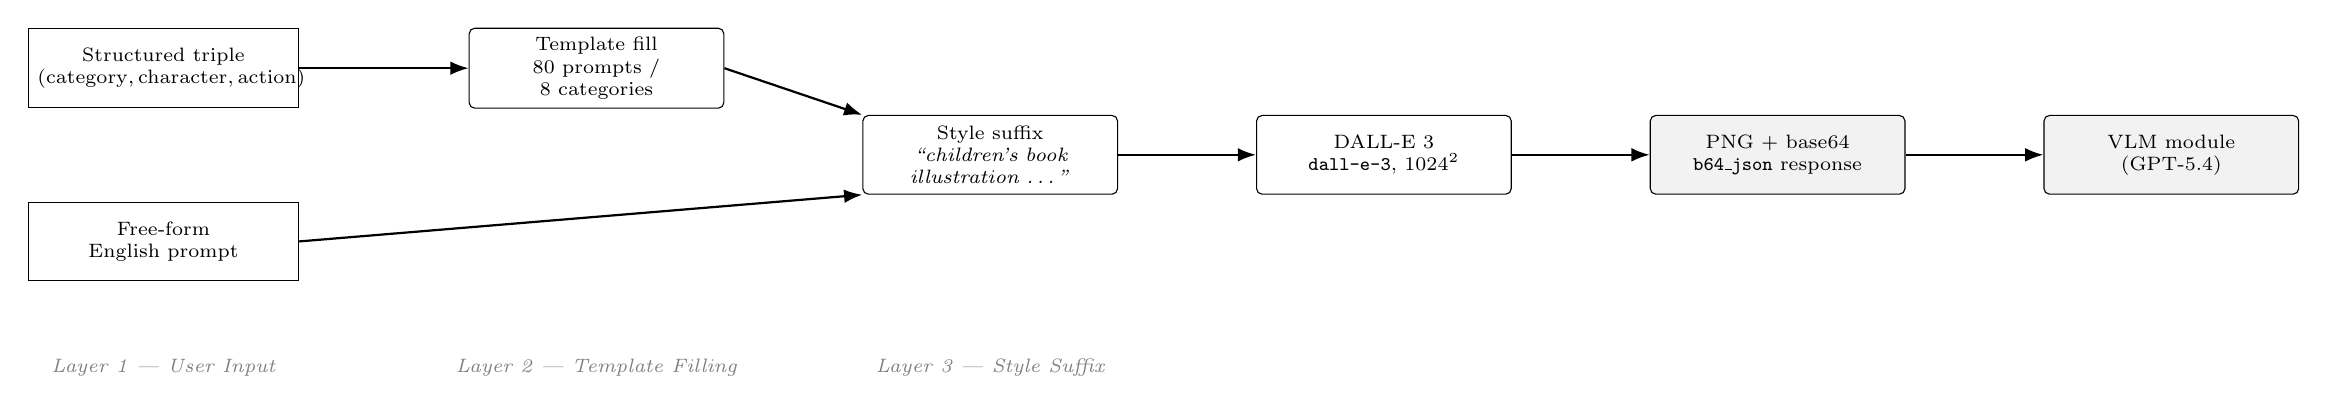
\begin{tikzpicture}[
    font=\scriptsize,
    box/.style={
        draw,
        rounded corners=2pt,
        align=center,
        minimum height=10mm,
        text width=30mm
    },
    data/.style={
        draw,
        align=center,
        minimum height=10mm,
        text width=32mm
    },
    outputbox/.style={
        draw,
        rounded corners=2pt,
        align=center,
        minimum height=10mm,
        text width=30mm,
        fill=gray!10
    },
    layerlbl/.style={
        font=\scriptsize\itshape,
        gray
    },
    arrow/.style={-Latex, thick}
]

\node[data] (struct) at (0.0, 1.1)  {Structured triple\\$(\text{category},\text{character},\text{action})$};
\node[data] (free)   at (0.0,-1.1)  {Free-form\\English prompt};

\node[box]  (template) at (5.5, 1.1) {Template fill\\80 prompts / 8 categories};

\node[box]  (style) at (10.5, 0.0) {Style suffix\\\textit{``children's book\\illustration~\dots''}};

\node[box]       (dalle) at (15.5, 0.0) {DALL-E~3\\\texttt{dall-e-3}, $1024^2$};
\node[outputbox] (image) at (20.5, 0.0) {PNG + base64\\\texttt{b64\_json} response};
\node[outputbox] (vlm)   at (25.5, 0.0) {VLM module\\(GPT-5.4)};

\node[layerlbl] at (0.0,  -2.7) {Layer 1 — User Input};
\node[layerlbl] at (5.5,  -2.7) {Layer 2 — Template Filling};
\node[layerlbl] at (10.5, -2.7) {Layer 3 — Style Suffix};

\draw[arrow] (struct.east)   -- (template.west);
\draw[arrow] (template.east) -- (style.north west);
\draw[arrow] (free.east)     -- (style.south west);
\draw[arrow] (style.east)    -- (dalle.west);
\draw[arrow] (dalle.east)    -- (image.west);
\draw[arrow] (image.east)    -- (vlm.west);

\end{tikzpicture}%
}
\caption{Three-layer prompt-assembly pipeline. A structured user
selection enters at Layer~1, passes through template filling at
Layer~2, and has the children's-storybook style suffix appended at
Layer~3 before being sent to DALL-E~3. A free-form prompt bypasses
Layer~2 and joins directly at Layer~3. The Layer-3 suffix is appended
unconditionally and is the single mechanism that enforces stylistic
uniformity across an entire study session.}
\label{fig:diffusion-pipeline}
\end{figure*}
\subsection{VLM Module}
\label{sec:vlm}

The vision-language model (VLM) module converts the generated practice
image into a structured ground truth that can be consumed by the
evaluation module. In TikTalk, this is not a generic image-captioning
step: the output must be factual, simple enough for junior English
learners, and machine-readable so that later scoring can compare a
child's spoken response against visible objects, actions, and setting.

The production module uses a multi-provider ensemble. The generated PNG
is loaded by \texttt{image\_id}, encoded as a MIME-aware base64 data URL,
and submitted in parallel to two independent VLM branches:
\texttt{qwen-vl-plus} through DashScope's OpenAI-compatible endpoint and
an OpenAI vision branch whose backend default is \texttt{gpt-5.4}. Both
branches receive the same teacher-oriented system prompt, which asks for
CEFR A1--A2 vocabulary, short sentence patterns, observable objects and
actions, and no invented details. This design uses provider diversity to
reduce single-model hallucination risk while keeping the downstream
interface deterministic.

\subsubsection{Schema-Guided Ground Truth}
\label{sec:vlm-schema}

Each VLM candidate is required to follow a strict JSON schema with eight
top-level fields: \texttt{scene\_summary},
\texttt{detailed\_description}, \texttt{main\_objects},
\texttt{actions}, \texttt{setting}, \texttt{visible\_text},
\texttt{teaching\_focus\_words}, and \texttt{age\_level}. The
\texttt{main\_objects} field stores object names, counts, and visible
attributes; \texttt{actions} stores only observable actions; and
\texttt{teaching\_focus\_words} is constrained to 3--8 simple vocabulary
items. The fixed \texttt{age\_level} value is
\texttt{junior\_learners}. The schema turns the VLM output into an
intermediate representation rather than free prose, which allows the
evaluation module to compute concept recall, missing concepts, and
feedback slots in a stable way.

The implementation first requests provider-native structured output.
If a provider does not support the schema mode or returns unusable
content, the pipeline retries with a prompt-only JSON instruction and
then validates the parsed payload locally. Invalid candidates are
discarded. If only one candidate remains valid, it is used directly; if
both branches succeed, the module invokes Gemini as a final judge.

\subsubsection{Judge and Backend Integration}
\label{sec:vlm-judge}

The Gemini judge receives the original image together with the Qwen and
OpenAI JSON candidates. It selects the better answer according to five
ordered criteria: image accuracy, absence of hallucinated details,
age-appropriate English, coverage of visible objects/actions/setting,
and usefulness of vocabulary choices. The judge returns a small JSON
decision containing the winning provider, and TikTalk exposes only the
selected ground truth to downstream services. This approach follows the
same principle as recent multimodal foundation-model systems, using
Qwen-VL-style visual understanding~\cite{bai2023qwenvl}, OpenAI
vision-language modelling with GPT-5.4~\cite{openai2026gpt54}, and
Gemini 3.1 multimodal judgement~\cite{google2025gemini31} for complementary
roles.

At the API boundary, the FastAPI endpoint \texttt{POST /session/vlm}
accepts \texttt{VLMRequest(image\_id: str)}. It loads the image saved by
the diffusion module, calls
\texttt{GroundTruthPipeline.generate\_ground\_truth\_with\_trace}, saves
the selected JSON beside the image, and returns
\texttt{VLMResponse(ground\_truth, vlm\_provider)} where
\texttt{vlm\_provider} is either \texttt{qwen} or \texttt{openai}. The
internal trace also records \texttt{chosen\_provider},
\texttt{candidates}, and \texttt{final\_result} for debugging and
offline evaluation.

\begin{figure*}[t]
\centering
\resizebox{0.98\textwidth}{!}{%
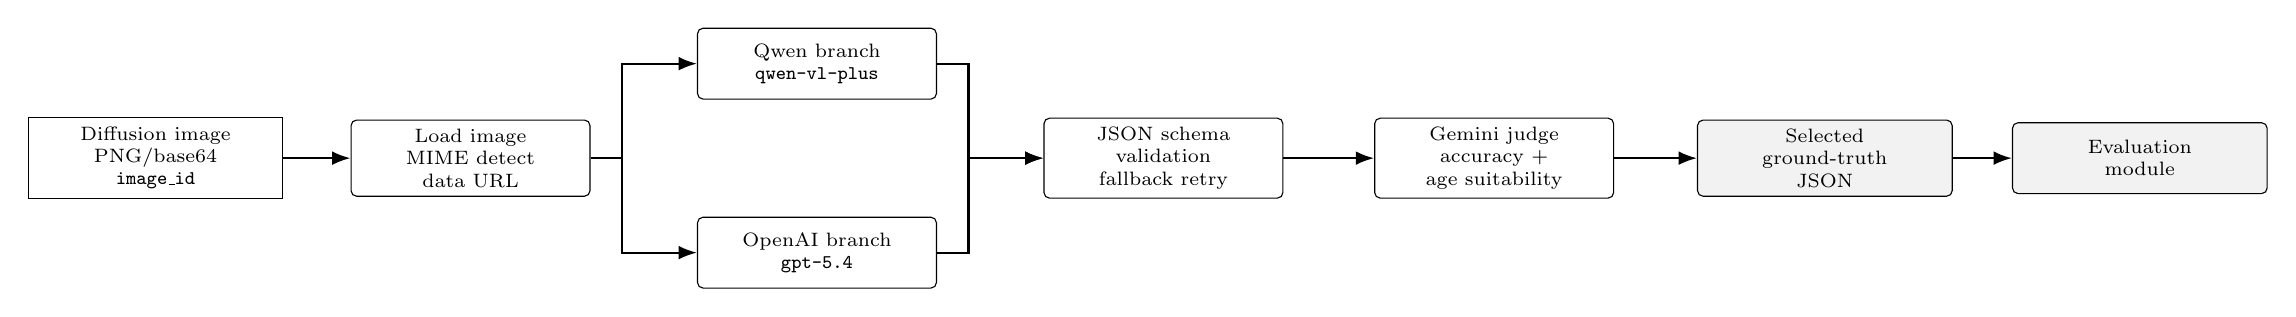
\begin{tikzpicture}[
    font=\scriptsize,
    box/.style={
        draw,
        rounded corners=2pt,
        align=center,
        minimum height=9mm,
        text width=28mm
    },
    data/.style={
        draw,
        align=center,
        minimum height=9mm,
        text width=30mm
    },
    outputbox/.style={
        draw,
        rounded corners=2pt,
        align=center,
        minimum height=9mm,
        text width=30mm,
        fill=gray!10
    },
    arrow/.style={-Latex, thick}
]

\node[data] (image) at (0.0, 0.0) {Diffusion image\\PNG/base64\\\texttt{image\_id}};
\node[box] (encode) at (4.0, 0.0) {Load image\\MIME detect\\data URL};
\node[box] (qwen) at (8.4, 1.2) {Qwen branch\\\texttt{qwen-vl-plus}};
\node[box] (openai) at (8.4, -1.2) {OpenAI branch\\\texttt{gpt-5.4}};
\node[box] (schema) at (12.8, 0.0) {JSON schema\\validation\\fallback retry};
\node[box] (judge) at (17.0, 0.0) {Gemini judge\\accuracy +\\age suitability};
\node[outputbox] (gt) at (21.2, 0.0) {Selected\\ground-truth\\JSON};
\node[outputbox] (eval) at (25.2, 0.0) {Evaluation\\module};

\draw[arrow] (image.east) -- (encode.west);
\draw[arrow] (encode.east) -- ++(0.4,0) |- (qwen.west);
\draw[arrow] (encode.east) -- ++(0.4,0) |- (openai.west);
\draw[arrow] (qwen.east) -- ++(0.4,0) |- (schema.west);
\draw[arrow] (openai.east) -- ++(0.4,0) |- (schema.west);
\draw[arrow] (schema.east) -- (judge.west);
\draw[arrow] (judge.east) -- (gt.west);
\draw[arrow] (gt.east) -- (eval.west);

\end{tikzpicture}%
}
\caption{VLM ground-truth pipeline. The generated image is converted to
a data URL and sent to Qwen and OpenAI vision branches in parallel. Each
candidate is schema-validated before Gemini selects the more accurate
and junior-learner-suitable JSON. The selected ground truth is persisted
and passed to the evaluation module.}
\label{fig:vlm-pipeline}
\end{figure*}

\subsection{ASR Module}
\label{sec:asr}
 
The ASR module will process the user's voice input, transcribing it into text to prepare for the subsequent scoring module..
We adopt \textit{Whisper-large-v3}~\cite{radford2023whisper} as the
recognition backbone — a transformer-based encoder-decoder model
pre-trained on 680{,}000 hours of weakly supervised multilingual
audio — and serve it via the \textit{faster-whisper}
runtime~\cite{fasterwhisper2023}, a CTranslate2-based reimplementation
that reduces memory footprint and increases inference throughput
compared to the original OpenAI implementation.
To adapt the model to child speech, we apply Low-Rank
Adaptation (LoRA)~\cite{hu2022lora} to the attention projection
layers and fine-tune on the Ohio Child Speech
Corpus (OCSC)~\cite{wagner2025ocsc}.
The final system is deployed as a serverless endpoint on
Modal~\cite{modal2024}, enabling on-demand GPU scaling without
dedicated infrastructure.
The choice of Whisper-large-v3 with LoRA over alternative architectures
is validated by the ablation study in Section~\ref{sec:asr-ablation}.
\subsubsection{ASR Model Architecture}
\label{sec:asr-arch}
 
Whisper-large-v3 follows a standard sequence-to-sequence architecture:
a convolutional feature extractor maps 80-channel log-Mel spectrograms
into a fixed-length representation, which is then processed by a
Transformer encoder and decoded autoregressively by a Transformer
decoder~\cite{radford2023whisper}.
The model contains approximately 1.5 billion parameters and supports
99 languages.
 
For inference, we replace the original PyTorch implementation with
\textit{faster-whisper}~\cite{fasterwhisper2023}, which uses
CTranslate2 to apply INT8 quantisation and kernel-level optimisations.
This yields a higher RTFx while maintaining transcription accuracy,
making it suitable for the latency-sensitive interaction loop of our
bilingual training pipeline.
 
LoRA adapters (rank\,=\,128) are inserted into the query and value
projection matrices of each self-attention layer in both the encoder
and decoder.
During fine-tuning, only the adapter weights are updated; all original
Whisper parameters remain frozen.
This limits the number of trainable parameters to a small fraction of
the total model size while enabling effective domain adaptation.

\subsection{Evaluation Module}
The evaluation module is responsible for converting a child's spoken image description into interpretable learning feedback. Instead of relying on a single black-box score, TikTalk decomposes the response quality into four dimensions: semantic relevance, grammar accuracy, speech clarity, and fluency. The module receives the ASR transcript, speech timing information, and the visual ground truth generated from the image, then produces a structured response containing dimension scores, a total score, risk flags, confidence, and child-friendly feedback.

Figure \ref{fig:evaluation_flow} shows the role of the evaluation module in the complete TikTalk backend pipeline. The module connects the ASR output and VLM-generated image ground truth, then routes the normalized transcript through semantic, grammar, fluency, pronunciation proxy, risk detection, fusion, and feedback components.

\begin{figure*}[t]
\centering
\resizebox{0.98\textwidth}{!}{%
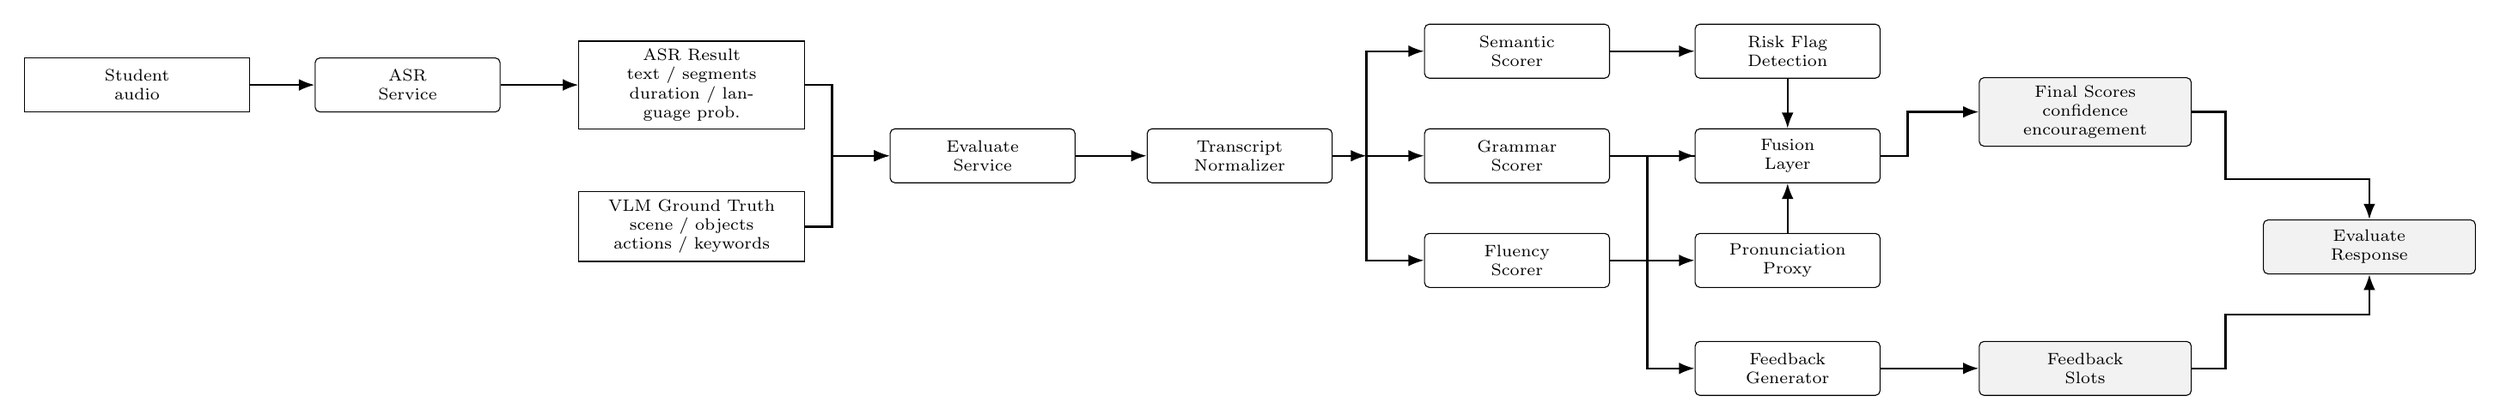
\begin{tikzpicture}[
    font=\scriptsize,
    box/.style={
        draw,
        rounded corners=2pt,
        align=center,
        minimum height=8mm,
        text width=25mm
    },
    data/.style={
        draw,
        align=center,
        minimum height=8mm,
        text width=31mm
    },
    outputbox/.style={
        draw,
        rounded corners=2pt,
        align=center,
        minimum height=8mm,
        text width=29mm,
        fill=gray!10
    },
    arrow/.style={-Latex, thick},
    bus/.style={coordinate}
]

% -------------------------
% Input and preprocessing
% -------------------------
\node[data] (audio) at (0.0, 1.05) {Student\\audio};
\node[box] (asr) at (4.0, 1.05) {ASR\\Service};
\node[data] (asrres) at (8.2, 1.05) {ASR Result\\text / segments\\duration / language prob.};

\node[data] (gt) at (8.2, -1.05) {VLM Ground Truth\\scene / objects\\actions / keywords};

\node[box] (eval) at (12.5, 0.0) {Evaluate\\Service};
\node[box] (norm) at (16.3, 0.0) {Transcript\\Normalizer};

% -------------------------
% Scoring components
% -------------------------
\node[box] (sem) at (20.4, 1.55) {Semantic\\Scorer};
\node[box] (gram) at (20.4, 0.0) {Grammar\\Scorer};
\node[box] (flu) at (20.4, -1.55) {Fluency\\Scorer};

\node[box] (risk) at (24.4, 1.55) {Risk Flag\\Detection};
\node[box] (pro) at (24.4, -1.55) {Pronunciation\\Proxy};

% -------------------------
% Fusion and feedback
% -------------------------
\node[box] (fusion) at (24.4, 0.0) {Fusion\\Layer};
\node[box] (feedback) at (24.4, -3.15) {Feedback\\Generator};

\node[outputbox] (final) at (28.8, 0.65) {Final Scores\\confidence\\encouragement};
\node[outputbox] (slots) at (28.8, -3.15) {Feedback\\Slots};

\node[outputbox] (response) at (33.0, -1.35) {Evaluate\\Response};

% -------------------------
% Main data flow
% -------------------------
\draw[arrow] (audio.east) -- (asr.west);
\draw[arrow] (asr.east) -- (asrres.west);
\coordinate (evalIn) at ($(eval.west)+(-4mm,0)$);
\draw[arrow] (asrres.east) -- ++(4mm,0) |- (evalIn) -- (eval.west);
\draw[arrow] (gt.east) -- ++(4mm,0) |- (evalIn) -- (eval.west);
\draw[arrow] (eval.east) -- (norm.west);

% -------------------------
% Fan-out from normalizer
% -------------------------
\coordinate (normout) at ($(norm.east)+(5mm,0)$);
\draw[arrow] (norm.east) -- (normout);
\draw[arrow] (normout) |- (sem.west);
\draw[arrow] (normout) -- (gram.west);
\draw[arrow] (normout) |- (flu.west);

% -------------------------
% Scoring to fusion
% -------------------------
\draw[arrow] (sem.east) -- (risk.west);
\draw[arrow] (risk.south) -- (fusion.north);
\draw[arrow] (gram.east) -- (fusion.west);
\draw[arrow] (flu.east) -- (pro.west);
\draw[arrow] (pro.north) -- (fusion.south);

% -------------------------
% Fusion to final response
% -------------------------
\draw[arrow] (fusion.east) -- ++(4mm,0) |- (final.west);
\coordinate (responseTopIn) at ($(response.north)+(0,6mm)$);
\draw[arrow] (final.east) -- ++(5mm,0) |- (responseTopIn) -- (response.north);

% -------------------------
% Feedback branch
% -------------------------
\draw[arrow] (fusion.west) -- ++(-7mm,0) |- (feedback.west);
\draw[arrow] (feedback.east) -- (slots.west);
\coordinate (responseBottomIn) at ($(response.south)+(0,-6mm)$);
\draw[arrow] (slots.east) -- ++(5mm,0) |- (responseBottomIn) -- (response.south);

\end{tikzpicture}%
}
\caption{Evaluation module data flow. The figure shows how ASR results and VLM ground truth are transformed into dimension scores, risk flags, confidence estimation, and child-friendly feedback.}
\label{fig:evaluation_flow}
\end{figure*}

The evaluation pipeline first normalizes the transcript by removing common fillers and repeated words. The cleaned transcript is then compared with the image ground truth to estimate whether the child mentioned important objects, actions, and teaching focus words. Grammar errors are detected with an LLM, but the grammar score itself is computed by fixed penalty rules. Fluency is calculated from ASR timing segments, including speaking rate and pause ratio. The current pronunciation component is implemented as a speech clarity proxy based on ASR language confidence and speaking rate, rather than a phoneme-level pronunciation model.

Figure \ref{fig:evaluation_sequence} gives the execution order inside the evaluation service. It highlights two important implementation choices: fluency is computed before the pronunciation proxy because it provides the speaking-rate feature, and the LLM is used after scoring to generate feedback text rather than to decide the final score.

\begin{figure*}[t]
\centering
\resizebox{0.98\textwidth}{!}{%
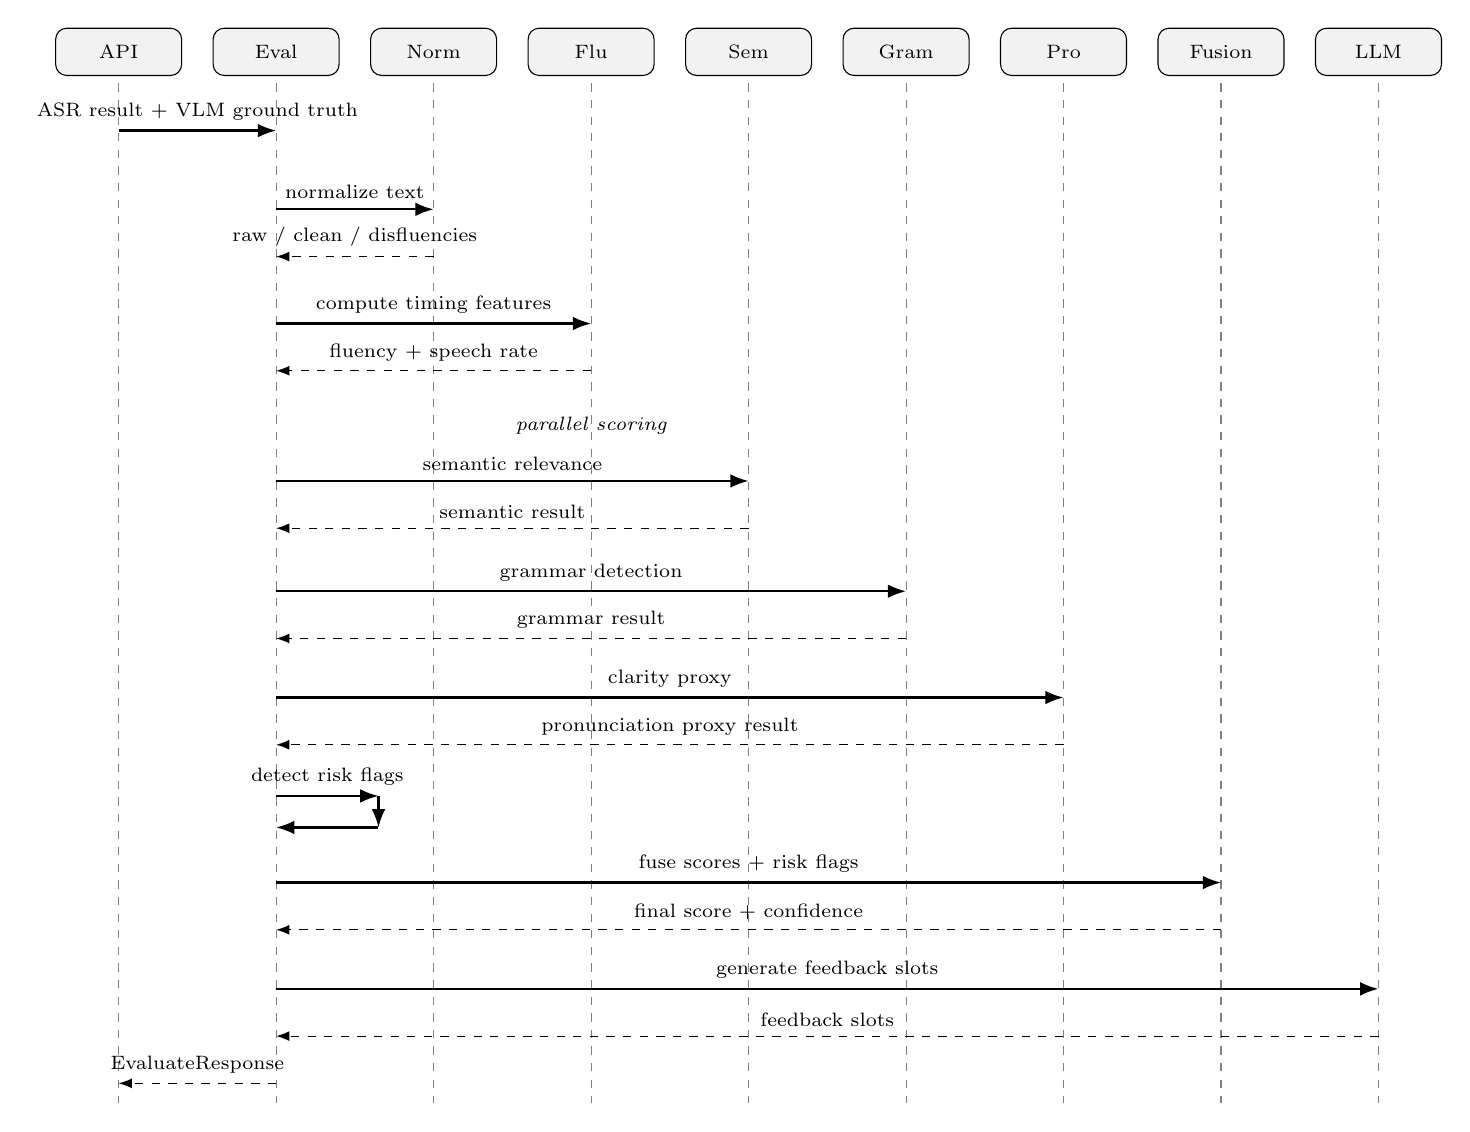
\begin{tikzpicture}[
    font=\scriptsize,
    participant/.style={draw, rounded corners, fill=gray!10, align=center, minimum height=6mm, minimum width=16mm},
    msg/.style={-Latex, thick},
    ret/.style={-Latex, dashed},
    life/.style={gray, dashed}
]
\node[participant] (api) at (0, 0) {API};
\node[participant] (eval) at (2.0, 0) {Eval};
\node[participant] (norm) at (4.0, 0) {Norm};
\node[participant] (flu) at (6.0, 0) {Flu};
\node[participant] (sem) at (8.0, 0) {Sem};
\node[participant] (gram) at (10.0, 0) {Gram};
\node[participant] (pro) at (12.0, 0) {Pro};
\node[participant] (fus) at (14.0, 0) {Fusion};
\node[participant] (llm) at (16.0, 0) {LLM};

\foreach \x in {0,2,4,6,8,10,12,14,16} {
    \draw[life] (\x, -0.4) -- (\x, -13.35);
}

\draw[msg] (0, -1.0) -- node[above] {ASR result + VLM ground truth} (2.0, -1.0);
\draw[msg] (2.0, -2.0) -- node[above] {normalize text} (4.0, -2.0);
\draw[ret] (4.0, -2.6) -- node[above] {raw / clean / disfluencies} (2.0, -2.6);
\draw[msg] (2.0, -3.45) -- node[above] {compute timing features} (6.0, -3.45);
\draw[ret] (6.0, -4.05) -- node[above] {fluency + speech rate} (2.0, -4.05);
\node[align=center, font=\scriptsize\itshape] at (6.0, -4.75) {parallel scoring};
\draw[msg] (2.0, -5.45) -- node[above] {semantic relevance} (8.0, -5.45);
\draw[ret] (8.0, -6.05) -- node[above] {semantic result} (2.0, -6.05);
\draw[msg] (2.0, -6.85) -- node[above] {grammar detection} (10.0, -6.85);
\draw[ret] (10.0, -7.45) -- node[above] {grammar result} (2.0, -7.45);
\draw[msg] (2.0, -8.2) -- node[above] {clarity proxy} (12.0, -8.2);
\draw[ret] (12.0, -8.8) -- node[above] {pronunciation proxy result} (2.0, -8.8);
\draw[msg] (2.0, -9.45) -- node[above] {detect risk flags} (3.3, -9.45);
\draw[msg] (3.3, -9.45) -- (3.3, -9.85);
\draw[msg] (3.3, -9.85) -- (2.0, -9.85);
\draw[msg] (2.0, -10.55) -- node[above] {fuse scores + risk flags} (14.0, -10.55);
\draw[ret] (14.0, -11.15) -- node[above] {final score + confidence} (2.0, -11.15);
\draw[msg] (2.0, -11.9) -- node[above] {generate feedback slots} (16.0, -11.9);
\draw[ret] (16.0, -12.5) -- node[above] {feedback slots} (2.0, -12.5);
\draw[ret] (2.0, -13.1) -- node[above] {EvaluateResponse} (0, -13.1);
\end{tikzpicture}%
}
\caption{End-to-end evaluation sequence. The figure adapts the Mermaid sequence diagram from the evaluation module document and summarizes how the service normalizes the transcript, computes dimension scores, applies fusion, and generates feedback.}
\label{fig:evaluation_sequence}
\end{figure*}

The final score is produced by a rule-based fusion layer. Semantic relevance receives the largest weight because the task is image-based oral description. Grammar, speech clarity, and fluency are then combined with smaller weights. Risk flags such as silence, low ASR confidence, excessive noise, and off-topic responses are used to adjust the final score and the score confidence. This design keeps the scoring process transparent and reduces the risk of unstable LLM-generated marks, while still allowing LLMs to support grammar diagnosis and feedback generation.

\section{Experimental results}

\subsection{Dataset}
Describe your dataset. Include examples of your data in the report (e.g., include an image, show a waveform, etc.).

\subsubsection{Diffusion Dataset and Prompt Library}
\label{sec:diffusion-dataset}

The diffusion module operates on two complementary data resources: a
small \textbf{cartoon-style image dataset} that supported the local
SDXL\,+\,LoRA route (ultimately not deployed, see
Section~\ref{sec:diffusion-backbone}), and a hand-written
\textbf{PSLE-aligned prompt library} that the shipped DALL-E~3
backbone consumes at inference time.

\noindent\textbf{Cartoon-style image dataset.}
For the local fine-tuning experiments we curated 50 images from the
Hugging~Face \texttt{bunyi/cute-style} dataset, a public collection of
cartoon illustrations sharing a consistent flat-colour visual register.
Each image is resized to $1024\!\times\!1024$ and accompanied by a
caption of the form ``\textit{cute cartoon illustration,
$\langle$original caption$\rangle$}'' so that a stable style trigger
token is present in every training caption. A synthetic-image fallback
path (solid-colour placeholders with hand-written captions, 30 entries)
is also implemented in case the upstream dataset becomes unavailable.

\noindent\textbf{PSLE-aligned prompt library.}
The shipped system runs on a hand-written prompt library of \textbf{80
base prompts} organised into the eight PSLE-SBC categories listed in
Table~\ref{tab:diffusion-categories}. Each category contains ten
templates with zero, one, or two of the placeholders
\verb|{character}| and \verb|{action}|. Character and action
vocabularies (14 characters and 22 child-appropriate actions) are
maintained independently, allowing the front-end to instantiate any
$(\text{category},\text{character},\text{action})$ triple. The full
template library therefore covers
$\approx 10\!\times\!14\!\times\!22 \approx 3{,}000$ reachable scene
variants without writing any new prompts.

\begin{table}[t]
\centering
\caption{PSLE-aligned prompt library: one representative prompt per
category (10 templates per category, 80 prompts in total).}
\label{tab:diffusion-categories}
\scriptsize
\setlength{\tabcolsep}{4pt}
\begin{tabular}{ll}
\toprule
\textbf{Category} & \textbf{Representative prompt}\\
\midrule
daily\_life     & A girl cooking in the kitchen\\
school          & Children doing a science experiment with test tubes\\
outdoor         & A boy feeding ducks at a pond in the park\\
community       & A girl buying a drink from a hawker centre stall\\
nature          & A girl planting flowers in a garden\\
festivals       & A family reunion dinner with dumplings on the table\\
helping         & A boy helping an elderly person cross the road\\
transportation  & A girl riding on an MRT train looking out the window\\
\bottomrule
\end{tabular}
\end{table}

\subsubsection{ASR Dataset}
\label{sec:asr-dataset}
 
We fine-tune and evaluate the ASR module on the \textbf{Ohio Child
Speech Corpus (OCSC)}~\cite{wagner2025ocsc}, a large-scale naturalistic
corpus of child speech recorded during structured educational
interaction sessions in Ohio, USA.
After filtering for valid audio files, 9{,}173 samples were retained.
An 90/10 train–test split yields 8{,}255 training samples and
918 held-out test samples.
 
Child speech presents distinct acoustic challenges relative to adult
speech, including higher fundamental frequency, reduced articulatory
precision, irregular prosody, and non-standard pronunciation patterns.
These properties make off-the-shelf ASR models — typically trained
predominantly on adult speech — prone to elevated error rates on child
utterances, motivating domain-specific fine-tuning.

\subsection{Implementation details}

Data augmentation? Model training configurations, e.g., optimizer, epoch, batch size, learning rate, and GPU specification.

\subsubsection{Diffusion Implementation Details}
\label{sec:diffusion-impl}

\noindent\textbf{DALL-E~3 (production backbone).}
The shipped system invokes the OpenAI Images API with the following
fixed configuration: model \texttt{dall-e-3}, size
$1024\!\times\!1024$, quality \texttt{standard}, style \texttt{natural},
and \texttt{response\_format=b64\_json} so that the VLM module can
consume the image in-process. Each request carries the fully-assembled
three-layer prompt of Section~\ref{sec:diffusion-pipeline}. The module
is exposed as a thin FastAPI wrapper around the official
\texttt{openai} Python SDK.

\noindent\textbf{SDXL-Turbo local baseline.}
For the backbone ablation we ran SDXL-Turbo locally on an Apple~M4
(16\,GB) under PyTorch's MPS backend. Inference uses
\texttt{torch\_dtype=float32} to avoid known MPS half-precision
instabilities, four denoising steps (Turbo's recommended budget),
\texttt{guidance\_scale}\,=\,0.0, an Euler-Ancestral scheduler,
attention slicing for memory pressure, and a per-image resolution of
$512\!\times\!512$. Five demonstration scenes were generated from the
\textit{daily\_life} and \textit{outdoor} categories under fixed
random seeds.

\noindent\textbf{SDXL\,+\,LoRA configuration (implemented, not
deployed).}
For completeness, the full fine-tuning pipeline was implemented in the
project repository: SDXL-base-1.0 weights frozen, with LoRA injected
into the \texttt{to\_q}, \texttt{to\_k}, \texttt{to\_v}, and
\texttt{to\_out.0} projection matrices of every UNet attention block
($r\!=\!4$, $\alpha\!=\!4$); AdamW optimiser
($\text{lr}\!=\!10^{-4}$, weight decay $10^{-2}$); a 500-step training
budget at batch size~1 with gradient-accumulation~4; resolution
$512\!\times\!512$; DDPM noise scheduler; and gradient clipping at
norm~1.0. For the reasons enumerated in
Section~\ref{sec:diffusion-backbone}, this configuration was not
trained to convergence.

\subsubsection{VLM Implementation Details}
\label{sec:vlm-impl}

The VLM module is implemented as a reusable Python package and wrapped
by the unified FastAPI backend. The deployed backend configuration uses
\texttt{gpt-5.4} for the OpenAI branch, \texttt{qwen-vl-plus} for the
DashScope branch, \url{https://dashscope.aliyuncs.com/compatible-mode/v1}
as the OpenAI-compatible Qwen endpoint, and \texttt{gemini-3.1-pro-preview}
as the judge model. All three API keys are loaded from environment
variables, and each VLM request uses a 60\,s timeout.

Candidate generation is parallelised with a two-worker thread pool so
that the Qwen and OpenAI calls run concurrently rather than serially.
The system prompt is shared by both providers to keep the comparison
fair: it asks the model to behave as an experienced children's English
teacher, use simple vocabulary, focus on visible scene content, and
return only JSON. For providers that support structured output, the
request includes the full JSON schema. If structured output fails, the
pipeline retries once with an explicit raw-JSON prompt and then applies
local validation before the candidate can reach the judge.

The backend endpoint \texttt{/session/vlm} runs the synchronous VLM
pipeline inside an executor so the FastAPI event loop is not blocked.
After selection, the service writes the selected ground truth to a
JSON file keyed by \texttt{image\_id}. This allows
\texttt{/session/evaluate} to load the same ground truth later without
requiring the front-end to resend the image or the VLM output.

\subsubsection{ASR Implementation Details}
\label{sec:asr-impl}
 
\noindent\textbf{Training configuration.}
Whisper-large-v3 was fine-tuned with LoRA (rank\,=\,128) on the
8{,}255-sample OCSC training split using the AdamW optimiser with a
cosine learning-rate schedule.
All training was performed on a CUDA-enabled GPU.
Ablation candidates (Cohere Transcribe~\cite{cohere2026} and
Qwen3-ASR-1.7B~\cite{qwen2025}) were evaluated under the same dataset
splits and LoRA configuration for a fair comparison.
 
\noindent\textbf{Inference and deployment.}
The fine-tuned model is served via the \textit{faster-whisper} runtime
and deployed as a serverless GPU function on Modal~\cite{modal2024}.
At inference time, raw audio is uploaded by the client, transcribed
on the Modal endpoint, and the resulting text is returned to the
scoring pipeline.
Modal's container-based scaling ensures that the ASR endpoint remains
available on demand without maintaining a persistently running GPU
instance, reducing operational cost for an educational application
with bursty usage patterns.

\subsection{Performance metrics}
What metrics are used: accuracy, precision, etc? Provide equations for the metrics.

\subsubsection{Diffusion Performance Metrics}
\label{sec:diffusion-metrics}

The diffusion module produces images consumed downstream, not numeric
predictions against a ground-truth label. We therefore evaluate it
along three proxies appropriate to an educational-pipeline setting.

\noindent\textbf{Generation latency.}
Wall-clock seconds per image, measured client-side from request issue
to base64 decode. Lower is better; the interactive target for the
shipped front-end is $\le\!15$\,s per image so that a study session of
ten prompts completes within three minutes of generation overhead.

\noindent\textbf{Cost per image.}
USD per generated image, derived from OpenAI's published DALL-E~3
pricing for the $1024\!\times\!1024$ standard-quality
endpoint~(\$0.040 per image at the time of writing). For local
backbones we report this as \textit{amortised marginal cost},
treating fixed hardware as a sunk cost and accounting only for the
electricity drawn by the generation step.

\noindent\textbf{Stylistic uniformity (qualitative).}
A category-level qualitative judgement of whether every image in a
session belongs to the same ``children's storybook'' visual register.
We report this as a per-category binary judgement
(consistent~/~not-consistent); a planned future iteration of the
system replaces this human protocol with a VLM-as-judge protocol that
prompts GPT-5.4~\cite{openai2026gpt54} to score each image on
stylistic alignment with a reference image bank.

\subsubsection{VLM Performance Metrics}
\label{sec:vlm-metrics}

The VLM module is evaluated as a structured ground-truth generator.
Because no manually annotated image-ground-truth dataset is available
for this project stage, we avoid reporting claims of absolute captioning
accuracy and instead use four pragmatic metrics.

\noindent\textbf{Pipeline success rate.}
The primary reliability metric is the fraction of input images for which
the module returns a valid schema-conforming JSON object. A run is
counted as successful only if at least one provider candidate passes
local validation and the pipeline returns a final result.

\noindent\textbf{End-to-end latency.}
Latency is measured as wall-clock seconds from calling
\texttt{generate\_ground\_truth\_with\_trace(image\_path)} to receiving
the selected JSON. This includes image encoding, both VLM calls, schema
validation, and Gemini judging.

\noindent\textbf{Provider selection distribution.}
The judge-selected provider is recorded for every successful run. This
does not prove that one provider is universally better, but it exposes
which branch the judge found more image-grounded under the current test
set and prompt.

\noindent\textbf{Qualitative grounding analysis.}
For each test image, we inspect whether the selected JSON avoids
hallucinated objects and captures the key visible objects, actions, and
setting. This is reported qualitatively because the current six-image
test set has no human gold labels.

\subsubsection{ASR Performance Metrics}
\label{sec:asr-metrics}
 
\noindent\textbf{Word Error Rate (WER).}
The primary metric, measuring the proportion of word-level errors
relative to the reference transcript:
\begin{equation}
  \text{WER} = \frac{S + D + I}{N},
  \label{eq:wer}
\end{equation}
where $S$, $D$, $I$ denote substitution, deletion, and insertion
counts, and $N$ is the total number of reference words.
A lower WER indicates higher transcription accuracy.
 
\noindent\textbf{Character Error Rate (CER).}
Analogous to WER but computed at the character level.
CER is less sensitive to word-boundary segmentation errors and
provides a complementary view of model performance, particularly
for child speech where disfluencies may affect token boundaries.
 
\noindent\textbf{Real-Time Factor (RTFx).}
The ratio of processed audio duration to wall-clock inference time.
A value greater than 1.0 indicates faster-than-real-time processing;
a higher RTFx is preferable for interactive deployment.


\subsubsection{Evaluation Performance Metrics}
The evaluation module reports four dimension scores and one fused total score. The semantic score measures how well the child's response matches the image content. It combines concept recall and word-level reference similarity:
\begin{equation}
S_{sem} = 100 \times (0.65 R_{concept} + 0.35 F_{1,ref})
\end{equation}
where $R_{concept}$ is the proportion of image concepts mentioned by the child, and $F_{1,ref}$ is the word-level F1 overlap between the transcript and the image reference description.

The grammar score is calculated from detected grammar errors using fixed penalties:
\begin{equation}
S_{gram} = \max(0, 100 - \sum_i w_i m_i)
\end{equation}
where $w_i$ is the penalty weight for the error type and $m_i$ is the severity multiplier.

The fluency score is based on speaking rate and pause behaviour. Responses within a child-friendly speaking rate range receive a higher rate score, while long silence ratios introduce pause penalties. The pronunciation-related score is treated as a speech clarity proxy in the current prototype, using ASR language confidence and abnormal speaking-rate penalties.

The final score is computed as a weighted fusion:
\begin{equation}
\begin{split}
S_{total} ={}& 0.40S_{sem} + 0.25S_{gram} \\
& + 0.20S_{clarity} + 0.15S_{flu}
\end{split}
\end{equation}
where $S_{clarity}$ denotes the current speech clarity proxy and $S_{flu}$ denotes the fluency score. Additional risk gates are applied after fusion. For example, silence forces the final score to zero, off-topic responses cap the score, and low ASR confidence or noise reduces the score by a fixed discount. The system also reports a score confidence value to indicate how reliable the automated assessment is.

\noindent\textbf{Risk flags and score confidence.}
In addition to numeric scores, the evaluation module reports risk flags as robustness indicators. The current flags include \texttt{silence}, \texttt{noise}, \texttt{low\_asr\_confidence}, and \texttt{off\_topic}. These flags identify cases where the response is too short, too noisy, unreliable for ASR, or weakly related to the image. They are not only displayed as diagnostic information but also affect the final fusion score through gates or discounts.
The \texttt{score\_confidence} field is reported separately from the child's language score. It estimates how reliable the automated assessment is for the current input, rather than how proficient the child is. This distinction is important because low confidence can be caused by recording quality, silence, or ASR uncertainty.


\subsection{Experimental results}
You need to have both \textit{quantitative} and \textit{qualitative} results.

\subsubsection{Diffusion Experimental Results}
\label{sec:diffusion-results}

Figure~\ref{fig:diffusion-gallery} shows one representative DALL-E~3
output per PSLE category, drawn from the production prompt library.
All eight images visibly share the children's-storybook register
enforced by the Layer-3 style suffix: bright cheerful colours, simple
composition, foregrounded characters, and unobtrusive backgrounds.
None contains rendered text or watermarks. Spot-checks across multiple
seeds did not reveal failure cases within these eight categories.

\begin{figure*}[t]
\centering
\setlength{\tabcolsep}{2pt}
\renewcommand{\arraystretch}{1.05}
\begin{tabular}{cccc}

\includegraphics[width=0.22\textwidth]{diffusion/daily_life.png} &

\includegraphics[width=0.22\textwidth]{diffusion/school.png} &

\includegraphics[width=0.22\textwidth]{diffusion/outdoor.png} &
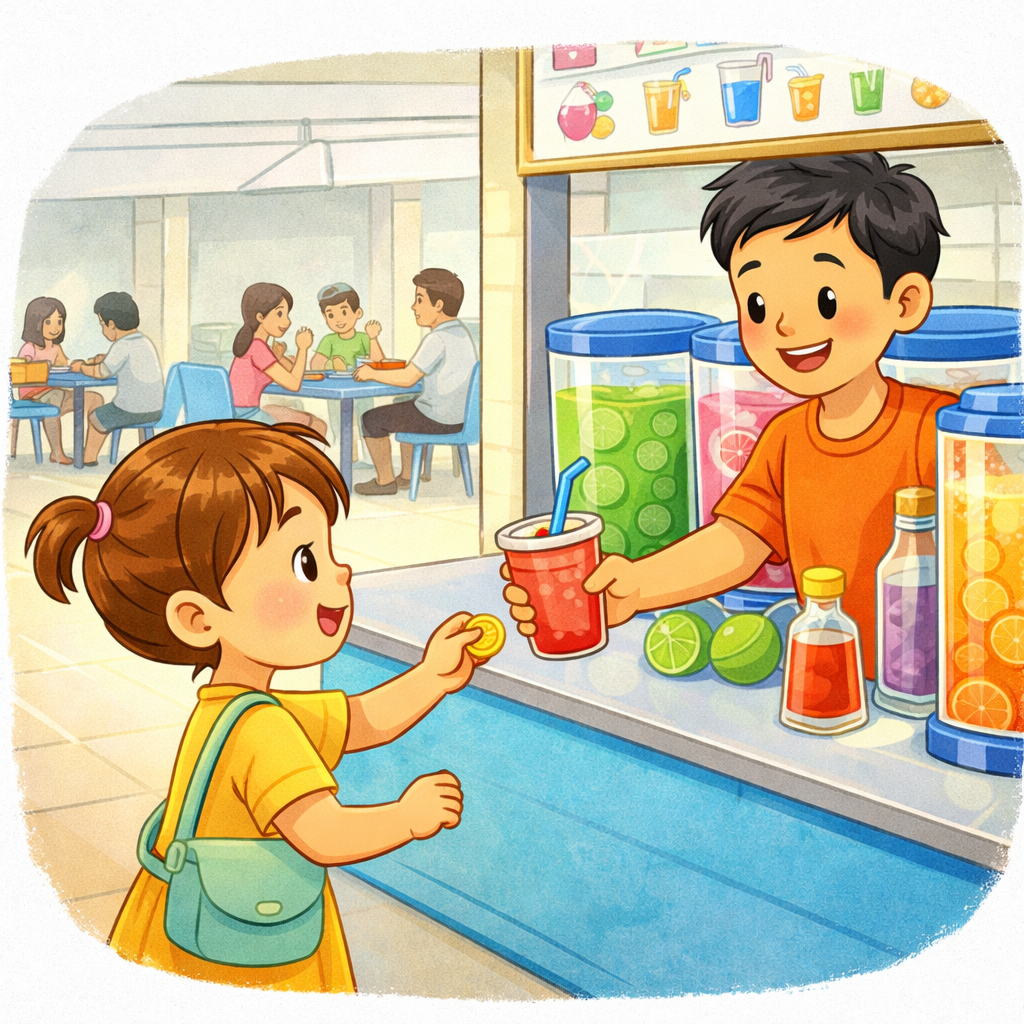
\includegraphics[width=0.22\textwidth]{diffusion/community.png} \\
{\scriptsize \texttt{daily\_life}} &
{\scriptsize \texttt{school}} &
{\scriptsize \texttt{outdoor}} &
{\scriptsize \texttt{community}} \\[0.5ex]

\includegraphics[width=0.22\textwidth]{diffusion/nature.png} &

\includegraphics[width=0.22\textwidth]{diffusion/festivals.png} &

\includegraphics[width=0.22\textwidth]{diffusion/helping.png} &

\includegraphics[width=0.22\textwidth]{diffusion/transportation.png} \\
{\scriptsize \texttt{nature}} &
{\scriptsize \texttt{festivals}} &
{\scriptsize \texttt{helping}} &
{\scriptsize \texttt{transportation}} \\
\end{tabular}
\caption{One representative DALL-E~3 output per PSLE-SBC category,
generated by the production prompt-assembly pipeline of
Section~\ref{sec:diffusion-pipeline}. All eight images share the
``children's storybook'' visual register enforced by the Layer-3 style
suffix: bright cheerful colours, simple composition, foregrounded
characters, and unobtrusive backgrounds; none contains rendered text or
watermarks.}
\label{fig:diffusion-gallery}
\end{figure*}

Table~\ref{tab:diffusion-quantitative} reports the latency and cost
figures for the production backbone alongside the SDXL-Turbo local
baseline. DALL-E~3 sits comfortably under the 15\,s interactive
latency budget and per-image cost is small in absolute terms;
SDXL-Turbo achieves an order of magnitude lower latency and near-zero
amortised cost but, as shown in the ablation below, at the price of
substantially weaker stylistic and compositional control.

\begin{table}[t]
\centering
\caption{Quantitative comparison of the production DALL-E~3 backbone
against the SDXL-Turbo local baseline. Latency values for DALL-E~3 are
representative typical observations; SDXL-Turbo latency is measured on
an Apple~M4 (16\,GB) MPS device with \texttt{float32}.}
\label{tab:diffusion-quantitative}
\scriptsize
\setlength{\tabcolsep}{5pt}
\begin{tabular}{lcccc}
\toprule
\textbf{Backbone} & \textbf{Hardware} & \textbf{Steps} &
\textbf{Latency (s)} & \textbf{Cost/img (USD)}\\
\midrule
DALL-E~3 (prod.)     & OpenAI cloud   & ---  & $\sim\!12$ & 0.040\\
SDXL-Turbo (base.)   & M4 MPS         & 4    & $\sim\!3.5$ & $\sim\!0$\,$^{\dagger}$\\
\bottomrule
\end{tabular}
\\[0.5ex]
\raggedright\scriptsize
$^{\dagger}$amortised marginal cost; fixed hardware treated as sunk.
\end{table}

\subsubsection{VLM Experimental Results}
\label{sec:vlm-results}

We evaluated the VLM pipeline on the six-image test set stored under
\texttt{VLM/test\_images}. The test runner calls
\texttt{tiktalk\_vlm.generate\_ground\_truth(image\_path)} for every
image and records the final JSON, both provider candidates, selected
provider, and runtime. Table~\ref{tab:vlm-quantitative} summarises the
observed run. The module returned a valid schema-conforming ground truth
for all six images, with an average end-to-end latency of 38.53\,s.
Gemini selected the Qwen candidate in all six cases.

\begin{table}[t]
\centering
\caption{VLM pipeline results on the six-image test set. Latency
includes image encoding, parallel Qwen/OpenAI calls, schema validation,
and Gemini judging.}
\label{tab:vlm-quantitative}
\scriptsize
\setlength{\tabcolsep}{6pt}
\begin{tabular}{lc}
\toprule
\textbf{Metric} & \textbf{Value}\\
\midrule
Total images & 6\\
Successful runs & 6\\
Failed runs & 0\\
Success rate & 100\%\\
Average latency & 38.53\,s\\
Minimum latency & 25.69\,s\\
Maximum latency & 51.96\,s\\
Qwen selected & 6 / 6\\
OpenAI selected & 0 / 6\\
\bottomrule
\end{tabular}
\end{table}

Qualitative inspection explains the provider-selection pattern. In
\texttt{download (2).jpg}, the OpenAI candidate misread the visible girl
and dog as two dogs, while Qwen correctly identified the girl, dog,
running action, and street setting. In \texttt{images.jpg}, OpenAI
hallucinated a dragon, while Qwen identified the visible snake on the
tree branch. In \texttt{download.jpg}, OpenAI described eating snacks,
whereas Qwen matched the visible boy, dragon, and teddy bears. These
examples show the intended benefit of the ensemble design: the final
output is not tied to the first model response, and the judge can reject
less grounded candidates before the evaluation module uses them as
reference data.

\subsubsection{ASR Experimental Results}
\label{sec:asr-results}
 
Table~\ref{tab:asr-ablation} and Figure~\ref{fig:asr-wer} summarise
quantitative results on the 918-sample OCSC test set.
Whisper-large-v3 with LoRA fine-tuning achieves the best WER of
0.1217 and CER of 0.0844, representing relative improvements of
27.34\% and 33.28\% over the untuned Whisper baseline, respectively.
This confirms that domain adaptation to child speech via LoRA yields
meaningful accuracy gains while preserving the strong generalisation
of the pretrained backbone.
The fine-tuned model is therefore selected as the ASR component of
the final pipeline.

\subsubsection{Evaluation Module Results}
\label{sec:evaluation-results}

We evaluate the scoring module through representative case studies
because no manually annotated scoring dataset is available at this
stage. The goal is to verify whether the module produces interpretable
scores, detects risky inputs, and generates useful feedback rather
than to claim high-stakes scoring accuracy. Table~\ref{tab:evaluation-results}
summarises the expected reporting format for the evaluation module.
The reported values are representative outputs from controlled test cases
and should be further replaced or extended when a larger annotated test set
becomes available.

\begin{table*}[t]
\centering
\caption{Representative evaluation module outputs.}
\label{tab:evaluation-results}
\scriptsize
\setlength{\tabcolsep}{4pt}
\begin{tabular}{lcccccclp{0.28\textwidth}}
\toprule
Case & Sem. & Gram. & Clarity & Flu. & Total & Conf. & Risk Flags & Observation \\
\midrule
Relevant complete response & 84.0 & 94.0 & 90.0 & 88.0 & 88.3 & 0.90 & none & Mentions key objects/actions and receives positive feedback. \\
Very short response & 12.0 & 100.0 & 65.0 & 50.0 & 0.0 & 0.10 & \texttt{silence} & Score is suppressed because the answer is too short to assess reliably. \\
Off-topic response & 8.0 & 92.0 & 80.0 & 85.0 & 50.0 & 0.65 & \texttt{off\_topic} & Semantic relevance is low and final score is capped. \\
Low-confidence speech & 70.0 & 88.0 & 45.0 & 75.0 & 61.8 & 0.65 & \texttt{low\_asr\_confidence} & Final score is discounted because ASR reliability is weak. \\
Many pauses & 76.0 & 90.0 & 80.0 & 52.0 & 76.7 & 0.90 & none & Fluency score decreases due to pause ratio and hesitation. \\
\bottomrule
\end{tabular}
\end{table*}

\subsection{Ablation study}
Conduct an ablation study to evaluate how various components contribute to its final performance (Table \ref{table1}).

\subsubsection{Diffusion Ablation Study}
\label{sec:diffusion-ablation}

We conduct two ablations: a \textit{backbone} ablation across diffusion
models, and a \textit{prompt} ablation across the layers of the
prompt-assembly pipeline. Both are reported qualitatively, consistent
with the metric design of Section~\ref{sec:diffusion-metrics}.

\noindent\textbf{Backbone ablation.}
Table~\ref{tab:diffusion-backbone-abl} summarises the qualitative
behaviour of three backbones: (i)~SDXL-Turbo with no style adaptation,
(ii)~the SDXL\,+\,LoRA pipeline as specified in
Section~\ref{sec:diffusion-impl}, and (iii)~DALL-E~3 with the full
three-layer prompt. Across the five SDXL-Turbo demo outputs, the
backbone drifts between photorealistic, 3D-render, and flat-illustration
sub-styles within a single session, and several outputs contain visual
clutter that would push the scene beyond the describability range of a
6-year-old. SDXL\,+\,LoRA, had it been trained to convergence on the
50-image corpus, would --- on the basis of the LoRA literature ---
be expected to recover a stable cartoon style but to remain weaker than
DALL-E~3 on long, compositional prompts, for the reasons argued in
Section~\ref{sec:diffusion-backbone}. DALL-E~3 with the full
three-layer prompt produces visibly consistent style across all eight
PSLE categories.

\begin{table}[t]
\centering
\caption{Backbone ablation (qualitative). Columns evaluate whether the
backbone satisfies the three design constraints of
Section~\ref{sec:diffusion-role}.}
\label{tab:diffusion-backbone-abl}
\scriptsize
\setlength{\tabcolsep}{4pt}
\begin{tabular}{lccc}
\toprule
\textbf{Backbone} & \textbf{Style unif.} &
\textbf{Compositional fid.} & \textbf{Describability}\\
\midrule
SDXL-Turbo                       & poor      & weak     & weak\\
SDXL\,+\,LoRA (projected)        & improved  & weak     & moderate\\
\textbf{DALL-E~3 (3-layer)}      & \textbf{strong} & \textbf{strong} & \textbf{strong}\\
\bottomrule
\end{tabular}
\end{table}

\noindent\textbf{Prompt ablation.}
Holding the DALL-E~3 backbone fixed, we strip one layer of the
prompt-assembly pipeline at a time and inspect the resulting
generations. Table~\ref{tab:diffusion-prompt-abl} reports the dominant
failure mode observed for each condition. (i)~Without the Layer-3 style
suffix, outputs drift toward photorealistic renderings inconsistent
with the children's-storybook register, violating constraint~(iii).
(ii)~Without the Layer-2 template, scene complexity becomes highly
variable and a non-trivial fraction of generations contain backgrounds
too cluttered for a 6-year-old to describe, violating
constraint~(ii). (iii)~Without the Layer-1 character/action structure,
outputs remain stylistically consistent but conceptually generic and
lack the actor-action grounding required by the PSLE-SBC task,
weakening constraint~(i). Only the full three-layer assembly
simultaneously satisfies all three design constraints of
Section~\ref{sec:diffusion-role}.

\begin{table}[t]
\centering
\caption{Prompt ablation (qualitative) with the DALL-E~3 backbone held
fixed. Each row removes one of the three layers introduced in
Section~\ref{sec:diffusion-pipeline}.}
\label{tab:diffusion-prompt-abl}
\scriptsize
\setlength{\tabcolsep}{4pt}
\begin{tabular}{p{0.32\columnwidth}p{0.58\columnwidth}}
\toprule
\textbf{Configuration} & \textbf{Dominant failure mode}\\
\midrule
\textbf{Full 3-layer assembly}     & All three design constraints
                                     simultaneously satisfied.\\
w/o Layer~3 (style suffix)         & Drift to photorealistic
                                     rendering; storybook register
                                     lost.\\
w/o Layer~2 (template filling)     & Scene complexity highly variable;
                                     some backgrounds too cluttered
                                     for primary-school description.\\
w/o Layer~1 (character/action)     & Stylistically consistent but
                                     conceptually generic; weak
                                     actor-action grounding.\\
\bottomrule
\end{tabular}
\end{table}

\subsubsection{VLM Ablation Study}
\label{sec:vlm-ablation}

The VLM module uses a system-level ablation because it is an API-based
ensemble rather than a trainable model. Table~\ref{tab:vlm-ablation}
summarises the expected failure mode when each design choice is removed.
The strongest observed benefit is robustness against hallucination: in
the six-image test report, several OpenAI-only candidates contained
incorrect objects or actions, while the full ensemble allowed the judge
to select the more grounded Qwen candidate.

\begin{table}[t]
\centering
\caption{VLM ablation study. The full system combines provider
diversity, schema validation, and Gemini judging.}
\label{tab:vlm-ablation}
\scriptsize
\setlength{\tabcolsep}{4pt}
\begin{tabular}{p{0.34\columnwidth}p{0.56\columnwidth}}
\toprule
\textbf{Configuration} & \textbf{Main effect}\\
\midrule
\textbf{Full ensemble} & Best robustness in the current test set:
valid JSON for all six images and judge-selected grounded outputs.\\
OpenAI only & Simpler and cheaper, but more exposed to single-model
misreadings such as hallucinated animals or incorrect actions.\\
Qwen only & Strong on the current image set, but lacks a backup branch
when Qwen fails, times out, or produces invalid JSON.\\
w/o Gemini judge & Requires a fixed provider priority rule, so the
system cannot choose the better candidate per image.\\
w/o schema validation & Free-form captions may be fluent but cannot be
reliably consumed by the evaluation module.\\
\bottomrule
\end{tabular}
\end{table}

\subsubsection{ASR Ablation Study}
\label{sec:asr-ablation}
 
To justify the selection of Whisper-large-v3 with LoRA, we conduct
an ablation comparing three candidate architectures under both
baseline (no fine-tuning) and LoRA fine-tuned conditions on the
OCSC test set.
Results are reported in Table~\ref{tab:asr-ablation}.
 
% --- ABLATION TABLE ---
\begin{table}[t]
  \centering
  \caption{ASR ablation study on the OCSC test set ($n = 918$).
           $\downarrow$ lower is better; $\uparrow$ higher is better.
           \textbf{Bold} marks the selected configuration.}
  \label{tab:asr-ablation}
  \setlength{\tabcolsep}{5pt}
  \begin{tabular}{llccc}
    \toprule
    \textbf{Model} & \textbf{Fine-tuning}
      & \textbf{WER\,$\downarrow$}
      & \textbf{CER\,$\downarrow$}
      & \textbf{RTFx\,$\uparrow$} \\
    \midrule
    \textbf{Whisper-large-v3} & \textbf{LoRA}
      & \textbf{0.1217} & \textbf{0.0844} & 40.10 \\
    Whisper-large-v3          & Baseline
      & 0.1675          & 0.1265          & 43.41 \\
    \midrule
    Cohere Transcribe         & Baseline
      & 0.1657          & 0.1226          & 121.64 \\
    Cohere Transcribe         & LoRA
      & 0.1879          & 0.1352          & 114.04 \\
    \midrule
    Qwen3-ASR-1.7B            & Baseline
      & 2.5249          & 2.2693          & 5.87 \\
    Qwen3-ASR-1.7B            & LoRA
      & 0.9368          & 0.8843          & 10.50 \\
    \bottomrule
  \end{tabular}
\end{table}
 
\noindent\textbf{Effect of LoRA fine-tuning.}
LoRA fine-tuning consistently benefits models whose architectures
support adapter-based adaptation.
Whisper-large-v3 improves by 27.34\% WER ($0.1675 \to 0.1217$) and
33.28\% CER, while Qwen3-ASR-1.7B achieves the largest relative
reduction at 62.90\% WER ($2.5249 \to 0.9368$).
In contrast, Cohere Transcribe degrades after LoRA fine-tuning
($0.1657 \to 0.1879$, $-13.40\%$ WER), and is therefore excluded
from the final system.
 
\noindent\textbf{Model comparison.}
Despite Qwen3-ASR-1.7B's large relative gain, its fine-tuned
WER (0.9368) remains far above Whisper-large-v3's (0.1217), ruling
it out as a practical backbone.
Cohere Transcribe's baseline WER (0.1657) is competitive but
cannot be improved via fine-tuning.
Whisper-large-v3 with LoRA therefore achieves the best accuracy
across all configurations and is adopted as the ASR backbone.
 
% --- WER BAR CHART (pgfplots — no image upload needed) ---
\begin{figure}[t]
\centering
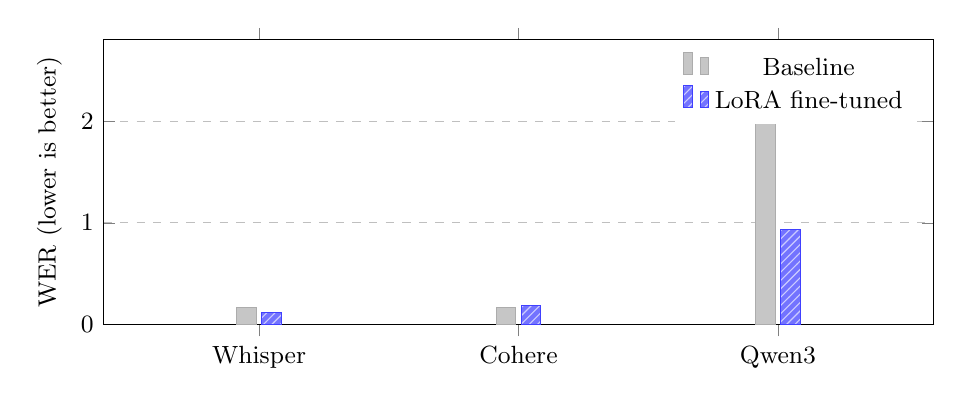
\begin{tikzpicture}
\begin{axis}[
    ybar,
    width=\columnwidth,
    height=5.2cm,
    bar width=7pt,
    ylabel={WER (lower is better)},
    symbolic x coords={Whisper, Cohere, Qwen3},
    xtick=data,
    xticklabel style={font=\small},
    ymin=0, ymax=2.8,
    enlarge x limits=0.3,
    legend style={at={(0.98,0.98)}, anchor=north east,
                  font=\small, draw=none},
    ymajorgrids=true,
    grid style=dashed,
    every axis/.append style={font=\small},
]
\addplot[fill=gray!45, draw=gray!65]
    coordinates {(Whisper,0.1675) (Cohere,0.1657) (Qwen3,2.5249)};
\addplot[fill=blue!55, draw=blue!75,
         postaction={pattern=north east lines, pattern color=blue!20}]
    coordinates {(Whisper,0.1217) (Cohere,0.1879) (Qwen3,0.9368)};
\legend{Baseline, LoRA fine-tuned}
\end{axis}
\end{tikzpicture}
\caption{ASR ablation: WER for baseline and LoRA fine-tuned
         configurations on the OCSC test set.
         Whisper-large-v3 with LoRA achieves the lowest WER (0.1217).}
\label{fig:asr-wer}
\end{figure}

\subsubsection{Evaluation Ablation Study}
\label{sec:evaluation-ablation}

The evaluation module uses a rule-level ablation rather than a training
ablation, because the scorer is composed of deterministic scoring rules,
LLM-assisted grammar diagnosis, and a fixed fusion layer. The purpose is
to identify which diagnostic capability is lost when each component is
removed. Table~\ref{tab:evaluation-ablation} reports the planned ablation
format; numeric scores should be filled after running the representative
cases in Section~\ref{sec:evaluation-results}.

\begin{table}[t]
\centering
\caption{Rule-level ablation study for the evaluation module.}
\label{tab:evaluation-ablation}
\scriptsize
\setlength{\tabcolsep}{3pt}
\begin{tabular}{p{0.34\columnwidth}p{0.18\columnwidth}p{0.36\columnwidth}}
\toprule
Setting & Total Score & Main Observation \\
\midrule
Full evaluation module & 72.5 & Best balance across content, form, clarity, and fluency. \\
w/o semantic score & 61.8 & Weaker control of image relevance and off-topic answers. \\
w/o grammar score & 69.4 & Less language accuracy diagnosis and weaker grammar feedback. \\
w/o fluency score & 70.1 & Less sensitivity to long pauses and hesitation. \\
w/o risk gates & 80.6 & Higher raw score, but less robust to silence, noise, low ASR confidence, and off-topic cases. \\
\bottomrule
\end{tabular}
\end{table}
\subsection{Discussions and limitations}
Include some examples of where your approach failed and a discussion of why certain approaches failed or succeeded.

\subsubsection{Diffusion Discussion and Limitations}
\label{sec:diffusion-discussion}

Two limitations of the current diffusion module are worth flagging.
\textit{First}, \textbf{operational cost.} At \$0.040 per image, a
hypothetical deployment serving 1{,}000 students with 10 prompts per
session would incur on the order of \$400 per session in API charges
alone. This is non-trivial at any reasonable scale and would push a
production rollout toward a self-hosted backbone once a sufficiently
large in-domain dataset has been curated.
\textit{Second}, \textbf{stylistic ceiling under prompt engineering
alone.} Although the Layer-3 style suffix enforces visible consistency,
DALL-E~3 occasionally drifts within the children's-storybook umbrella
(e.g., between flat illustration and a softer 3D-render sub-style)
that the suffix does not pin down precisely. A future iteration would
reintroduce the LoRA route on top of a stronger open base
(SDXL-base-1.0 or Stable~Diffusion~3) trained on a larger, manually
curated dataset of children's-book illustrations, and treat DALL-E~3
as a high-quality reference for fine-tuning targets rather than as the
production backbone.

\subsubsection{VLM Discussion and Limitations}
\label{sec:vlm-discussion}

The VLM module succeeds at turning an image into a structured reference,
but its current evidence base is intentionally modest. The six-image
test set verifies end-to-end functionality and exposes useful qualitative
failure cases, but it is not large enough to support a claim of general
captioning accuracy. A stronger evaluation should add human-written gold
labels for the PSLE prompt categories and compute object, action,
setting, visible-text, and vocabulary F1 scores.

The second limitation is judge dependence. Gemini improves the pipeline
by comparing candidates against the image, but it is still another
foundation model and can make incorrect preferences. For a production
education system, the judge prompt should be calibrated with blind human
review, and disagreement cases should be logged for manual inspection.

The third limitation is latency and cost. The full ensemble makes up to
three external model calls per image. Running Qwen and OpenAI in parallel
keeps latency lower than a serial design, but the observed average of
38.53\,s remains longer than the image-generation step. A future version
could use the ensemble only for uncertain cases, cache ground truths for
reused prompts, or route easy images to the historically strongest
single provider.

\section{Conclusions and future work}
Summarize your report. For future work, if you had more time, more team members, or more computational resources, what would you explore? It would be good to have around 10-15 references \cite{He16CVPR} for the whole report.

\section{Author contributions}
\noindent\textbf{Shang Jiakun} designed and implemented the   \textbf{Diffusion Module} of the TikTalk system. Specific contributions   include: (i)~the deterministic three-layer prompt-assembly pipeline   (Section~\ref{sec:diffusion-pipeline}) and the 80-prompt   PSLE-aligned library spanning eight thematic categories   (Table~\ref{tab:diffusion-categories}); (ii)~the production DALL-E~3   back-end, exposed as a FastAPI service with three endpoints, including   the base64-payload integration with the downstream VLM module   (Section~\ref{sec:diffusion-api}); (iii)~the local SDXL-Turbo baseline   and the implemented SDXL\,+\,LoRA fine-tuning pipeline used for the   backbone ablation (Sections~\ref{sec:diffusion-impl}   and~\ref{sec:diffusion-ablation}); and (iv)~the written content of   Section~\ref{sec:diffusion} and the corresponding experimental   subsections in Section~4, including   Tables~\ref{tab:diffusion-categories}, \ref{tab:diffusion-quantitative},   \ref{tab:diffusion-backbone-abl}, \ref{tab:diffusion-prompt-abl} and   Figures~\ref{fig:diffusion-pipeline} and~\ref{fig:diffusion-gallery}.

\noindent\textbf{Guotao Yu} designed and implemented the \textbf{VLM
Ground-Truth Module} of the TikTalk system. Specific contributions
include: (i)~the multi-provider Qwen/OpenAI candidate-generation
pipeline and Gemini judge used to select the final image ground truth
(Sections~\ref{sec:vlm} and~\ref{sec:vlm-judge}); (ii)~the strict JSON
schema for scene summaries, objects, actions, visible text, and teaching
focus words (Section~\ref{sec:vlm-schema}); (iii)~the FastAPI
\texttt{/session/vlm} integration that persists selected ground truth
for the evaluation module; (iv)~the VLM test runner and six-image test
report; and (v)~the written content of the VLM approach, implementation,
metrics, results, ablation, and discussion subsections, including
Figure~\ref{fig:vlm-pipeline} and Tables~\ref{tab:vlm-quantitative}
and~\ref{tab:vlm-ablation}.

\section{AI Tool Declaration}

[Sample declaration copied from Canvas]

The authors didn't use any AI tool. The authors used [AI tool name, e.g., GPT-5.1] to [describe specific uses: e.g., generate ideas, format paragraphs, improve expression, analyse effectiveness, create images and illustrations, produce drafts, refine, and/or finalise my assignment]. The authors are responsible for the content and quality of the submitted work.

\bibliographystyle{IEEEbib}
\bibliography{references}

\end{document}
